% College Lecture 5 topics not in the Neso videos: multiplicative/affine and its attack, cryptanalysis of Vigenere
% (Kasiski, index of coincidence) and Hill, rotor/Enigma, keyless/keyed/columnar transposition, stream vs block.
% Sources: Lecture 5 slides (scanned; OCR in scratchpad/r3/l5.txt), Forouzan ch. 3, Stallings ch. 2-3.
% Every number recomputed by script (scratchpad/r3/verify2.py, kas2.py).
\section{Traditional Ciphers: Remaining Topics (Lecture 5)}\label{sec:classextra}
The college lecture follows Forouzan's chapter 3, which treats the classical ciphers as arithmetic in $\mathbb{Z}_{26}$ (letters $a = 0, \dots, z = 25$) and pays more attention to how each cipher is \emph{broken}. This section collects what the Neso videos did not cover: the multiplicative and affine ciphers and the attack on them, the cryptanalysis of Vigen\`ere and Hill, rotor machines, Forouzan's family of transposition ciphers with their attacks, and the stream/block classification. Throughout, Eve knows the algorithm (Kerckhoff's principle, \S\ref{sec:attacks}) and only the key is secret.

\subsection{Multiplicative and affine ciphers \hot}
\asked{Mid-sem 2024--25 Q1(a,b): one plaintext change alters only \textbf{1} ciphertext character in multiplicative and affine ciphers (each letter is enciphered on its own).}
The additive (shift) cipher has only 26 keys, one of them useless, so it falls to brute force. The obvious variation is to \emph{multiply} instead of add. In the \textbf{multiplicative cipher} the plaintext and ciphertext are integers in $\mathbb{Z}_{26}$ and the key $k$ is an integer in $\mathbb{Z}_{26}^*$:
\[
C = (P \times k) \bmod 26, \qquad P = (C \times k^{-1}) \bmod 26 .
\]

\textbf{Why the key must be in $\mathbb{Z}_{26}^*$.} Encryption must be one-to-one, otherwise two plaintext letters share a ciphertext letter and Bob cannot tell which was sent. If $d = \gcd(k, 26) > 1$, then $P$ and $P + 26/d$ encrypt to the same letter, since $k(P + 26/d) = kP + 26 \cdot (k/d) \equiv kP$. With $k = 2$, for example, \ttx{a} ($0$) and \ttx{n} ($13$) both become \ttx{A}, and \ttx{b} and \ttx{o} both become \ttx{C}. If $\gcd(k, 26) = 1$, $k$ has a multiplicative inverse $k^{-1}$ modulo 26 (extended Euclid, \S\ref{sec:exteuclid}), so multiplying by $k^{-1}$ undoes the encryption. The usable keys are therefore exactly the elements of
\[
\mathbb{Z}_{26}^* = \{1, 3, 5, 7, 9, 11, 15, 17, 19, 21, 23, 25\}
\]
(the odd numbers except 13), and there are $\phi(26) = \phi(2)\phi(13) = 1 \times 12 = 12$ of them (\S\ref{sec:totient}). The key domain is even smaller than the additive one.

\textbf{The affine cipher} combines the two: the first key multiplies, the second adds,
\[
C = (P \times k_1 + k_2) \bmod 26, \qquad P = \big((C - k_2) \times k_1^{-1}\big) \bmod 26 ,
\]
where $k_1 \in \mathbb{Z}_{26}^*$ and $k_2 \in \mathbb{Z}_{26}$. Decryption reverses the two steps in the opposite order: adding the additive inverse $-k_2$ undoes the addition, and multiplying by $k_1^{-1}$ undoes the multiplication. The additive cipher is the special case $k_1 = 1$ and the multiplicative cipher the case $k_2 = 0$.

\textbf{Why the affine key space is 312.} $k_1$ can be any of the 12 elements of $\mathbb{Z}_{26}^*$ and $k_2$ any of the 26 elements of $\mathbb{Z}_{26}$, giving $12 \times 26 = 312$ pairs. No two pairs give the same substitution: if $(k_1, k_2)$ and $(k_1', k_2')$ encrypted every letter identically, then $P = 0$ would give $k_2 = k_2'$ and $P = 1$ would then give $k_1 = k_1'$. So the affine cipher has exactly 312 keys (311 excluding the identity $(1, 0)$; a script check finds 312 distinct substitution tables). This is a tiny subset of the $26!$ monoalphabetic substitutions: brute force over 312 keys is trivial, and since each letter always maps to the same letter, the cipher also keeps the English letter frequencies.

\textbf{One plaintext change changes one ciphertext letter.} Each letter is enciphered on its own, with the same key and without reference to its neighbours, so changing $P_i$ changes $C_i$ and nothing else. This holds for the additive, multiplicative and affine ciphers alike.

\begin{center}\small
\begin{tabular}{@{}lll@{}}
\toprule
Cipher & Encrypt & Decrypt / key space\\
\midrule
Additive (shift) & $C = (P + k) \bmod 26$ & $P = (C - k) \bmod 26$; \; 26 keys\\
Multiplicative & $C = (P \times k) \bmod 26$ & $P = (C \times k^{-1}) \bmod 26$; \; $k \in \mathbb{Z}_{26}^*$: \textbf{12 keys}\\
Affine & $C = (P k_1 + k_2) \bmod 26$ & $P = ((C - k_2) k_1^{-1}) \bmod 26$; \; $12 \times 26 = \mathbf{312}$ keys\\
\bottomrule
\end{tabular}
\end{center}

\begin{mustknow}[: multiplicative and affine]
$k$ (or $k_1$) must be in $\mathbb{Z}_{26}^* = \{1,3,5,7,9,11,15,17,19,21,23,25\}$, i.e.\ $\gcd(k, 26) = 1$, so that $k^{-1}$ exists. Inverses: $3 \leftrightarrow 9$, $5 \leftrightarrow 21$, $7 \leftrightarrow 15$, $11 \leftrightarrow 19$, $17 \leftrightarrow 23$, $1$ and $25$ are their own.\\
Key spaces: additive 26, multiplicative 12, affine $12 \times 26 = 312$. Two plaintext/ciphertext pairs determine an affine key.
\end{mustknow}

\begin{worked}[: Forouzan, ``hello'' with the multiplicative and affine ciphers]
\textbf{Q.} (a) Encrypt ``hello'' with the multiplicative cipher, key 7. (b) Encrypt ``hello'' with the affine cipher, key pair $(7, 2)$. (c) Decrypt \ttx{ZEBBW} with the key pair $(7, 2)$.

Since $\gcd(7, 26) = 1$, both keys are valid; $7^{-1} \bmod 26 = 15$ because $7 \times 15 = 105 = 4 \times 26 + 1$, and the additive inverse of 2 is $-2 \equiv 24$.
\begin{center}\small
\begin{tabular}{@{}cc|cc|ccc@{}}
\toprule
Letter & $P$ & $7P$ & (a) mod 26 & $7P + 2$ & mod 26 & (b) $C$\\
\midrule
h & 7 & 49 & 23 \ttx{X} & 51 & 25 & \ttx{Z}\\
e & 4 & 28 & 2 \ttx{C} & 30 & 4 & \ttx{E}\\
l & 11 & 77 & 25 \ttx{Z} & 79 & 1 & \ttx{B}\\
l & 11 & 77 & 25 \ttx{Z} & 79 & 1 & \ttx{B}\\
o & 14 & 98 & 20 \ttx{U} & 100 & 22 & \ttx{W}\\
\bottomrule
\end{tabular}
\end{center}
(a) \textbf{\ttx{XCZZU}}. \quad (b) \textbf{\ttx{ZEBBW}}.

(c) $P = (C - 2) \times 15 \bmod 26$:
\begin{center}\small
\begin{tabular}{@{}cc|ccc|c@{}}
\toprule
Cipher & $C$ & $C - 2$ & $\times 15$ & mod 26 & Plain\\
\midrule
Z & 25 & 23 & 345 & 7 & h\\
E & 4 & 2 & 30 & 4 & e\\
B & 1 & $-1$ & $-15$ & 11 & l\\
B & 1 & $-1$ & $-15$ & 11 & l\\
W & 22 & 20 & 300 & 14 & o\\
\bottomrule
\end{tabular}
\end{center}
Plaintext \textbf{hello} \checkmark. The doubled \ttx{l} gives a doubled \ttx{B}: the cipher is monoalphabetic.
\end{worked}

\subsection{Breaking the affine cipher: two pairs give $(k_1, k_2)$}
Brute force and frequency analysis both work on an affine ciphertext, but the cipher's linearity allows something faster. Each known plaintext/ciphertext letter pair $(P, C)$ gives one linear congruence in the two unknowns,
\[
P \times k_1 + k_2 \equiv C \pmod{26}.
\]
Two pairs give two congruences, and subtracting them eliminates $k_2$:
\[
(P_1 - P_2)\, k_1 \equiv C_1 - C_2 \pmod{26}.
\]
If $\gcd(P_1 - P_2, 26) = 1$, multiplying by $(P_1 - P_2)^{-1}$ gives a unique $k_1$, and then $k_2 = C_1 - P_1 k_1 \bmod 26$. The same solution in matrix form, as on the slides, is $\binom{k_1}{k_2} = \left(\begin{smallmatrix} P_1 & 1\\ P_2 & 1\end{smallmatrix}\right)^{-1} \binom{C_1}{C_2}$. Finally the candidate must be checked: a $k_1$ outside $\mathbb{Z}_{26}^*$ cannot be an affine key, which means the data did not come from an affine cipher (or one of the pairs is wrong). If $\gcd(P_1 - P_2, 26) = 2$, the congruence has two solutions $k_1$ and $k_1 + 13$ (or none); one of them is even and is rejected, so normally one key remains. Where the pairs come from decides the name of the attack: \emph{chosen-plaintext} if Eve types the plaintext herself, \emph{known-plaintext} if she merely learns it, and \emph{ciphertext-only} if she guesses that the two most frequent ciphertext letters stand for \ttx{e} and \ttx{t}.

\begin{worked}[: slide example, chosen-plaintext attack on the affine cipher]
\textbf{Q.} Eve intercepts \ttx{PWUFFOGWCHFDWIWEJOUUNJORSMDWRHVCMWJUPVCCG}. She briefly gets access to Alice's computer and has time to type only ``et''. She is not sure which of two algorithms is the affine cipher: algorithm 1 gives \ttx{WC}, algorithm 2 gives \ttx{WF}. Find the key and the plaintext.

\textbf{Algorithm 1} ($\ttx{e} = 4 \to \ttx{W} = 22$, $\ttx{t} = 19 \to \ttx{C} = 2$):
\[
4k_1 + k_2 \equiv 22, \qquad 19k_1 + k_2 \equiv 2 \pmod{26}.
\]
Subtract: $15k_1 \equiv 2 - 22 = -20 \equiv 6$. Since $15^{-1} = 7$ ($15 \times 7 = 105 = 4 \times 26 + 1$), $k_1 = 6 \times 7 = 42 \bmod 26 = 16$, and $k_2 = 22 - 4 \times 16 = -42 \equiv 10$. In matrix form: $\det\left(\begin{smallmatrix}4 & 1\\ 19 & 1\end{smallmatrix}\right) = 4 - 19 = -15 \equiv 11$, $11^{-1} = 19$, inverse $= 19\left(\begin{smallmatrix}1 & -1\\ -19 & 4\end{smallmatrix}\right) \equiv \left(\begin{smallmatrix}19 & 7\\ 3 & 24\end{smallmatrix}\right)$, and $\left(\begin{smallmatrix}19 & 7\\ 3 & 24\end{smallmatrix}\right)\binom{22}{2} = \binom{432}{114} \equiv \binom{16}{10}$. \textbf{Rejected}: $\gcd(16, 26) = 2$, so 16 has no inverse in $\mathbb{Z}_{26}^*$ (indeed $16 \times 0 \equiv 16 \times 13 \equiv 0$), and algorithm 1 is not the affine cipher.

\textbf{Algorithm 2} ($\ttx{t} = 19 \to \ttx{F} = 5$): $15k_1 \equiv 5 - 22 = -17 \equiv 9$, so $k_1 = 9 \times 7 = 63 \bmod 26 = \mathbf{11}$ and $k_2 = 22 - 4 \times 11 = -22 \equiv \mathbf{4}$. The coefficient matrix is the same as for algorithm 1 (same plaintext ``et''), so with the same inverse: $\left(\begin{smallmatrix}19 & 7\\ 3 & 24\end{smallmatrix}\right)\binom{22}{5} = \binom{453}{186} \equiv \binom{11}{4}$. Accepted: $\gcd(11, 26) = 1$.

\textbf{Decrypt.} The decryption key is the pair of inverses $(k_1^{-1}, -k_2) = (19, 22)$, since $11 \times 19 = 209 = 8 \times 26 + 1$: $P = 19\,(C + 22) \bmod 26$. First letters: \ttx{P} $= 15$: $19 \times 37 = 703 \equiv 1 = $ \ttx{b}; \ttx{W} $= 22$: $19 \times 44 = 836 \equiv 4 = $ \ttx{e}; \ttx{U} $= 20$: $19 \times 42 = 798 \equiv 18 = $ \ttx{s}; \ttx{F} $= 5$: $19 \times 27 = 513 \equiv 19 = $ \ttx{t}. The whole text is \textbf{best time of the year is spring when flowers bloom}. Check: encrypting it with $(11, 4)$ gives the intercepted ciphertext \checkmark.
\end{worked}

\begin{worked}[: new, known pair with an even difference]
\textbf{Q.} An affine cipher encrypts ``go'' as \ttx{MA}. Find the key and decrypt \ttx{MAAXLESG}.

\textbf{Equations.} \ttx{g} $= 6 \to$ \ttx{M} $= 12$ and \ttx{o} $= 14 \to$ \ttx{A} $= 0$: $6k_1 + k_2 \equiv 12$ and $14k_1 + k_2 \equiv 0$. Subtracting the first from the second: $8k_1 \equiv -12 \equiv 14 \pmod{26}$.

\textbf{Solve.} $\gcd(8, 26) = 2$ divides 14, so divide everything by 2: $4k_1 \equiv 7 \pmod{13}$. $4^{-1} \bmod 13 = 10$ ($40 = 3 \times 13 + 1$), so $k_1 \equiv 70 \equiv 5 \pmod{13}$, i.e.\ $k_1 \in \{5, 18\}$ modulo 26. $18$ is even, hence not in $\mathbb{Z}_{26}^*$: $k_1 = \mathbf{5}$, and $k_2 = 12 - 6 \times 5 = -18 \equiv \mathbf{8}$.

\textbf{Decrypt} with $5^{-1} = 21$ ($105 = 4 \times 26 + 1$): $P = 21\,(C - 8) \bmod 26$.
\begin{center}\small
\begin{tabular}{@{}l*{8}{c}@{}}
\toprule
$C$ & M 12 & A 0 & A 0 & X 23 & L 11 & E 4 & S 18 & G 6\\
$21(C - 8)$ & 84 & $-168$ & $-168$ & 315 & 63 & $-84$ & 210 & $-42$\\
mod 26 & 6 & 14 & 14 & 3 & 11 & 20 & 2 & 10\\
$P$ & g & o & o & d & l & u & c & k\\
\bottomrule
\end{tabular}
\end{center}
Plaintext \textbf{good luck}. Check: $5 \times 6 + 8 = 38 \equiv 12 = $ \ttx{M} \checkmark.
\end{worked}

\subsection{Cryptanalysis of Vigen\`ere: Kasiski test and index of coincidence}
Vigen\`ere ciphers, like all polyalphabetic ciphers, do not preserve the frequency of characters: each plaintext letter is shifted by one of $m$ different amounts, so the peaks of English are spread out. Their weakness is the \emph{period}. Every $m$-th letter is shifted by the same key letter, so the ciphertext is really $m$ interleaved additive ciphers (\S\ref{sec:poly}). Cryptanalysis therefore has two parts: \textbf{finding the length $m$ of the key}, and then \textbf{finding the key itself}.

\textbf{The Kasiski test.} English repeats short fragments constantly (\ttx{the}, \ttx{ing}, \ttx{and}, \ttx{tion}). When the same fragment occurs twice at a distance that is a multiple of $m$, both occurrences line up with the same key letters, so they are enciphered identically and the ciphertext shows a repeated segment. The Kasiski test therefore searches the ciphertext for repeated segments of \textbf{at least three characters} and measures the distance $d$ between them; the cryptanalyst assumes that $m$ divides $d$. With several repeats at distances $d_1, d_2, \dots, d_n$, $m$ divides all of them, so
\[
m \mid \gcd(d_1, d_2, \dots, d_n).
\]
A chance repetition (two different plaintext fragments under different key letters that happen to give the same three ciphertext letters) is rare, which is why short repeats of one or two letters are ignored; a distance that does not share the common factor is treated as such a coincidence and left out of the gcd.

\textbf{Finding the key.} Once $m$ is known, the ciphertext is divided into $m$ pieces: piece $j$ holds letters $j, j + m, j + 2m, \dots$. All letters of one piece were shifted by the same key letter, so each piece is an additive cipher on a sample of English and is broken by the methods for the additive cipher: frequency analysis, or simply trying all 26 shifts. \imp{The whole ciphertext does not preserve the single-letter frequencies of the plaintext, but each piece does.} The deciphered pieces are then interleaved one character at a time to give the plaintext; if it does not make sense, another $m$ is tried.

\textbf{The index of coincidence} (Friedman) finds $m$ without needing repeats. The IC of a text of $N$ letters, in which letter $i$ occurs $f_i$ times, is the probability that two letters picked at random from it are equal:
\[
\text{IC} = \frac{\sum_{i} f_i (f_i - 1)}{N (N - 1)} .
\]
For English it is about $\sum p_i^2 \approx 0.066$ (0.0655 from the standard frequency table), while for uniformly random letters it is $1/26 \approx 0.038$. A monoalphabetic substitution only renames the letters, so it leaves the IC unchanged; a Vigen\`ere ciphertext mixes $m$ alphabets, so its IC falls towards 0.038 as $m$ grows. To find $m$, split the ciphertext into $m$ pieces for each candidate $m$ and average the pieces' IC: for the right $m$ (and its multiples) every piece is a single Caesar cipher and its IC jumps to about 0.066.

\begin{worked}[: slide example, Forouzan's Vigen\`ere ciphertext]
\textbf{Q.} Find the key length and the key of the 175-letter Vigen\`ere ciphertext
\begin{center}\small\ttfamily
LIOMWGFEGGDVWGHHCQUCRHRWAGWIOWQLKGZETKKMEVLWPCZVGTHVTSGXQOVGCSVETQLTJSU\\
MVWVEUVLXEWSLGFZMVVWLGYHCUSWXQHKVGSHEEVFLCFDGVSUMPHKIRZDMPHHBVWVWJWIXGF\\
WLTSHGJOUEEHHVUCFVGOWICQLTJSUXGLW
\end{center}
\textbf{Kasiski.} Repetitions of three-character segments (positions as on the slide, counted from 0):
\begin{center}\small
\begin{tabular}{@{}lccc@{}}
\toprule
String & First index & Second index & Difference\\
\midrule
JSU & 68 & 168 & 100\\
SUM & 69 & 117 & 48\\
VWV & 72 & 132 & 60\\
MPH & 119 & 127 & 8\\
\bottomrule
\end{tabular}
\end{center}
(\ttx{QLT}, \ttx{LTJ} and \ttx{TJS} also repeat at distance 100; they are part of the same repeated block \ttx{QLTJSU}.) $100 = 4 \cdot 25$, $48 = 4 \cdot 12$, $60 = 4 \cdot 15$, $8 = 4 \cdot 2$, so $\gcd = 4$ and $m \in \{1, 2, 4\}$; try $m = 4$ first.

\textbf{Index of coincidence} of the pieces for each candidate $m$:
\begin{center}\small
\begin{tabular}{@{}lcccccc@{}}
\toprule
$m$ & 1 & 2 & 3 & 4 & 5 & 6\\
\midrule
average IC of the $m$ pieces & 0.053 & 0.056 & 0.050 & \textbf{0.077} & 0.059 & 0.053\\
\bottomrule
\end{tabular}
\end{center}
Only $m = 4$ (and its multiple 8, IC 0.069) reaches the English level; the values exceed 0.066 because each piece is only 43--44 letters long. Both tests agree: $\mathbf{m = 4}$.

\textbf{Break each piece.} Piece C1 is letters 1, 5, 9, \dots, piece C2 letters 2, 6, 10, \dots:
\begin{center}\small
\begin{tabular}{@{}lllcc@{}}
\toprule
Piece & Most frequent & Shift if top $=$ \ttx{e} & Best shift (all 26 tried) & Key letter\\
\midrule
C1 & \ttx{G} (8 of 44) & 2 & 2 & \ttx{c}\\
C2 & \ttx{S} (8 of 44) & 14 & 14 & \ttx{o}\\
C3 & \ttx{H} (7 of 44) & 3 & 3 & \ttx{d}\\
C4 & \ttx{M}, \ttx{E}, \ttx{V} (6 each of 43) & 8 (if \ttx{M}) & 4 & \ttx{e}\\
\bottomrule
\end{tabular}
\end{center}
For C4 the single most frequent letter is ambiguous, so all 26 shifts are tried and the one whose output has the most English-like letter distribution wins: shift 4 turns \ttx{M}, \ttx{E}, \ttx{V} into \ttx{i}, \ttx{a}, \ttx{r}, three common letters. The key is \textbf{\ttx{code}} (2, 14, 3, 4). Interleaving the deciphered pieces gives the slide's plaintext: \emph{``Julius Caesar used a cryptosystem in his war, which is now referred to as Caesar cipher. It is a shift cipher with the key set to three. Each character in the plaintext is shifted three characters to create ciphertext.''} (The text the slide actually encrypted contained a few typos; see the corrections box.)
\end{worked}

\textbf{Why neither test works on the one-time pad.} Its key has no period, so repeated ciphertext segments are pure coincidences whose distances have no common factor, and every way of splitting the ciphertext gives pieces with the random IC of about 0.038.

\subsection{Cryptanalysis of Hill: known-plaintext}
\textbf{Why the Hill cipher resists the earlier attacks.} A brute-force attack on a Hill cipher is extremely difficult, because the key is an $m \times m$ matrix and each entry can take one of 26 values: the key domain has size $26^{m \times m}$ ($26^4 = 456\,976$ matrices for $m = 2$, of which $157\,248$ are invertible; $26^9 \approx 5.4 \times 10^{12}$ for $m = 3$). Statistical attacks fail too. Each ciphertext letter $C_j = P_1 k_{1j} + P_2 k_{2j} + \dots + P_m k_{mj}$ depends on \emph{all} $m$ letters of its block, so the same plaintext letter is enciphered differently depending on its neighbours, and Eve cannot run frequency analysis on single letters, digrams or trigrams. Only whole blocks of $m$ letters that repeat at block-aligned positions repeat in the ciphertext, and a plaintext rarely has many such repeats.

\textbf{Why it falls to a known-plaintext attack.} The cipher is \emph{linear}: every block satisfies $C = PK \pmod{26}$. Suppose Eve knows $m$ and has the plaintext/ciphertext pairs of at least $m$ distinct blocks (from the same message or from different ones). She writes the $m$ plaintext blocks as the rows of an $m \times m$ matrix $P$ and the corresponding ciphertext blocks as the rows of $C$. Because each row satisfies the cipher equation, the whole matrices satisfy $C = PK$, and if $P$ is invertible modulo 26 (i.e.\ $\gcd(\det P, 26) = 1$),
\[
\boxed{K = P^{-1} C \pmod{26}} .
\]
If $P$ is not invertible, Eve chooses a different set of $m$ pairs. If she does not know $m$, she tries $m = 2, 3, \dots$ (provided $m$ is not very large) and tests each candidate key on one more known block. With $K$ she computes $K^{-1}$ and reads every message encrypted with that key. The lesson carried into modern ciphers is that \textbf{linearity is fatal}: DES and AES add non-linear S-boxes precisely so that no such matrix equation exists.

\begin{worked}[: Stallings, $2 \times 2$ Hill from a known plaintext]
\textbf{Q.} The plaintext ``friday'' is encrypted with a $2 \times 2$ Hill cipher (row-vector convention $C = PK$) to give \ttx{PQCFKU}. Find the key.

\textbf{Pairs.} \ttx{fr} $(5, 17) \to$ \ttx{PQ} $(15, 16)$; \;\ttx{id} $(8, 3) \to$ \ttx{CF} $(2, 5)$; \;\ttx{ay} $(0, 24) \to$ \ttx{KU} $(10, 20)$. Use the first two:
\[
P = \begin{pmatrix} 5 & 17\\ 8 & 3\end{pmatrix}, \qquad C = \begin{pmatrix} 15 & 16\\ 2 & 5\end{pmatrix}.
\]
\textbf{Invert $P$.} $\det P = 5 \cdot 3 - 17 \cdot 8 = -121 \equiv 9 \pmod{26}$; $\gcd(9, 26) = 1$ and $9^{-1} = 3$ ($27 = 26 + 1$).
\[
P^{-1} = 3 \begin{pmatrix} 3 & -17\\ -8 & 5\end{pmatrix} = \begin{pmatrix} 9 & -51\\ -24 & 15\end{pmatrix} \equiv \begin{pmatrix} 9 & 1\\ 2 & 15\end{pmatrix}.
\]
\textbf{Key.}
\[
K = P^{-1}C = \begin{pmatrix} 9 \cdot 15 + 1 \cdot 2 & 9 \cdot 16 + 1 \cdot 5\\ 2 \cdot 15 + 15 \cdot 2 & 2 \cdot 16 + 15 \cdot 5\end{pmatrix} = \begin{pmatrix} 137 & 149\\ 60 & 107\end{pmatrix} \equiv \mathbf{\begin{pmatrix} 7 & 19\\ 8 & 3\end{pmatrix}}.
\]
\textbf{Check with the third pair:} $(0, 24) K = (24 \cdot 8,\ 24 \cdot 3) = (192, 72) \equiv (10, 20) = $ \ttx{KU} \checkmark.
\end{worked}

\begin{worked}[: slide example, $m = 3$]
\textbf{Q.} Eve knows $m = 3$ and has intercepted three plaintext/ciphertext block pairs (not necessarily from the same message): $(05, 07, 10) \to (03, 06, 00)$, $(13, 17, 07) \to (14, 16, 09)$, $(00, 05, 04) \to (03, 17, 11)$. Find $K$.
\[
P = \begin{pmatrix}5&7&10\\13&17&7\\0&5&4\end{pmatrix},\quad
C = \begin{pmatrix}3&6&0\\14&16&9\\3&17&11\end{pmatrix},\quad
\det P = 451 \equiv 9,\quad 9^{-1} = 3 .
\]
With the adjugate of $P$ reduced mod 26,
\[
\operatorname{adj} P \equiv \begin{pmatrix}7&22&9\\0&20&17\\13&1&20\end{pmatrix},\qquad
P^{-1} = 3 \cdot \operatorname{adj} P \equiv \begin{pmatrix}21&14&1\\0&8&25\\13&3&8\end{pmatrix},\qquad
K = P^{-1}C \equiv \begin{pmatrix}2&3&7\\5&7&9\\1&2&11\end{pmatrix}.
\]
(All entries mod 26, verified: $P P^{-1} \equiv I$ and $PK \equiv C$.) Now Eve has the key and can break any ciphertext encrypted with it.
\end{worked}

\subsection{Rotor ciphers and Enigma}
\textbf{Rotor cipher.} The one-time pad is not practical, but monoalphabetic substitution is far too weak. One step toward more secure encipherment is the \textbf{rotor cipher}: it uses the idea of monoalphabetic substitution, but \textbf{changes the mapping between plaintext and ciphertext characters after every character}. The mapping is realised by a \textbf{rotor}, a disc with one contact per letter on each face and a fixed internal wiring that connects each input contact to an output contact; the wiring is one permutation of the alphabet. After each character the rotor turns by one position, so every wire meets different letters and the next character is encrypted with a shifted permutation. The key is the initial position of the rotor (and the wiring itself if it is secret). Since the same letter is enciphered differently at different positions, the rotor cipher is \textbf{polyalphabetic}, and it is a stream cipher whose key stream is the sequence of rotor positions.

\begin{center}
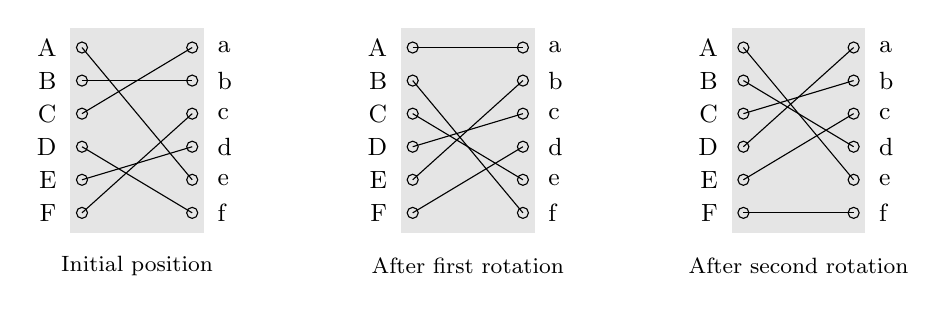
\begin{tikzpicture}[x=1cm,y=-0.42cm,font=\small]
\foreach \panel/\dx/\wires/\name in {0/0/{0/4,1/1,2/0,3/5,4/3,5/2}/Initial position, 1/4.2/{0/0,1/5,2/4,3/2,4/1,5/3}/After first rotation, 2/8.4/{0/4,1/3,2/1,3/0,4/2,5/5}/After second rotation}{
  \fill[gray!20] (\dx+0.25,-0.6) rectangle (\dx+1.95,5.6);
  \foreach \L [count=\i from 0] in {A,B,C,D,E,F}{\node[anchor=east] at (\dx+0.2,\i) {\L}; \draw (\dx+0.4,\i) circle (2pt);}
  \foreach \L [count=\i from 0] in {a,b,c,d,e,f}{\node[anchor=west] at (\dx+2.0,\i) {\L}; \draw (\dx+1.8,\i) circle (2pt);}
  \foreach \l/\r in \wires {\draw (\dx+0.4,\l) -- (\dx+1.8,\r);}
  \node[font=\footnotesize] at (\dx+1.1,6.6) {\name};
}
\end{tikzpicture}
\end{center}
\textbf{Example} (the slide's 6-letter rotor; plaintext on the right, ciphertext on the left). In the initial position \ttx{b} is wired to \ttx{B} and \ttx{e} to \ttx{A}; after the first rotation \ttx{e} is wired to \ttx{C}; after the second, \ttx{e} is wired to \ttx{A} again. If the rotor were stationary (a monoalphabetic substitution), ``bee'' would be encrypted as \ttx{BAA}. With the rotor turning after each letter it becomes \ttx{BCA}: the two \ttx{e}'s are encrypted as different characters. A single rotor of 26 contacts repeats its sequence of permutations every 26 letters, which is still a short period.

\textbf{The Enigma machine} was invented by Arthur Scherbius in 1918 for businesses that needed to send confidential documents without codebooks; it was modified by the German army and used extensively in World War II. It is based on the principle of rotor ciphers, with three rotors connected so that the \textbf{wiring changes as you type}. Its main parts are:
\begin{itemize}[leftmargin=1.4em]
  \item a \textbf{keyboard} for typing the plaintext and a \textbf{lampboard} on which the ciphertext letter lights up;
  \item a \textbf{plugboard} that swaps chosen pairs of letters on the way in and again on the way out;
  \item three \textbf{rotors}: the \emph{fast} rotor turns one position with every key press, the \emph{middle} rotor turns once per revolution of the fast rotor, and the \emph{slow} rotor once per revolution of the middle one (like the wheels of an odometer), so the sequence of substitutions repeats only after about $26^3 = 17\,576$ letters;
  \item a \textbf{reflector}, which sends the current back through the three rotors by a different path.
\end{itemize}
\begin{center}
\begin{tikzpicture}[node distance=8mm]
  \node[box,fill=cyan!10] (kb) {Keyboard};
  \node[box,fill=gray!15,right=of kb] (pb) {Plugboard};
  \node[box,fill=orange!15,right=of pb] (f) {Fast\\rotor};
  \node[box,fill=orange!15,right=of f] (m) {Middle\\rotor};
  \node[box,fill=orange!15,right=of m] (s) {Slow\\rotor};
  \node[box,fill=magenta!10,right=of s] (r) {Reflector};
  \node[box,fill=yellow!20,below=7mm of kb] (lb) {Lampboard};
  \foreach \a/\b in {kb/pb,pb/f,f/m,m/s,s/r}{\draw[arr,acc] ([yshift=1.6mm]\a.east) -- ([yshift=1.6mm]\b.west);}
  \foreach \a/\b in {r/s,s/m,m/f,f/pb}{\draw[arr,warn] ([yshift=-1.6mm]\a.west) -- ([yshift=-1.6mm]\b.east);}
  \draw[arr,warn] (pb.south) |- (lb.east);
  \node[font=\footnotesize,acc,above=1mm of f.north east] {forward};
  \node[font=\footnotesize,warn,below=1mm of m.south] {back, by another path};
\end{tikzpicture}
\end{center}
In the slide's example the key \ttx{T} is pressed: the plugboard turns it into \ttx{K}, the three wheels carry it to the reflector, which returns it on another contact, the wheels carry it back to \ttx{W}, and the plugboard turns \ttx{W} into \ttx{G}, so lamp \ttx{G} lights.

\textbf{Consequences of the reflector.} The current path is reversible, so with the same settings pressing \ttx{G} lights \ttx{T}: encryption and decryption are the same operation, which made the machine convenient. But the reflector never connects a contact to itself, so the return path always ends on a different letter: \textbf{Enigma never encrypts a letter to itself}. This was a real weakness. Allied cryptanalysts used it to place a guessed plaintext word (a \emph{crib}) against the ciphertext, rejecting every position where some letter would have mapped to itself, and then searched the rotor settings with machines (the \emph{bombes}). The key of a day was the choice and order of the rotors, their ring settings and starting positions, and the plugboard pairs.

\subsection{Transposition: keyless, keyed, combined \hot}
\asked{Mid-sem 2024--25 Q3(b): ``abcdefghij'' $\to$ ``CABDEHFGIJ'' with a keyed transposition: the pattern repeats every 5 letters, so the permutation key has size \textbf{5}.}
A transposition cipher does not substitute one symbol for another; it changes the location of the symbols (\S\ref{sec:transp}). Forouzan sorts transposition ciphers by how the permutation is produced.

\textbf{Keyless transposition.} Simple transposition ciphers used in the past are keyless: the permutation comes from the shape of a table, not from a key. There are two methods. In the first, the text is written into a table \emph{column by column} and transmitted \emph{row by row}; the rail fence is this method with a 2-row table. To send ``meet me at the park'', Alice writes the letters in a zig-zag over two lines and sends the first line followed by the second: \textbf{\ttx{MEMATEAKETETHPR}}. Bob divides the ciphertext in half (here the second half, \ttx{ETETHPR}, has one character fewer than the first, \ttx{MEMATEAK}), uses the halves as the two rows and reads in zig-zag. In the second method, the text is written \emph{row by row} and transmitted \emph{column by column}. With an agreed 4 columns Alice writes \ttx{meet|meat|thep|ark} and sends \textbf{\ttx{MMTAEEHREAEKTTP}}; Bob writes the ciphertext column by column and reads it row by row.

The permutation of the second method has a visible pattern. Writing each plaintext position under the ciphertext position it moves to,
\begin{center}\small\setlength{\tabcolsep}{3.5pt}
\begin{tabular}{@{}l*{15}{c}@{}}
\toprule
Plaintext position & 01&02&03&04&05&06&07&08&09&10&11&12&13&14&15\\
Ciphertext position & 01&05&09&13&02&06&10&14&03&07&11&15&04&08&12\\
\bottomrule
\end{tabular}
\end{center}
the second character has moved to the fifth position, the third to the ninth, and so on. The permutation falls into runs $(01, 05, 09, 13)$, $(02, 06, 10, 14)$, $(03, 07, 11, 15)$, $(04, 08, 12)$, in each of which adjacent numbers differ by 4, the number of rows. Such regularity is what the pattern attack below exploits.

\textbf{Keyed (block) transposition.} Instead of permuting the whole text at once, the plaintext is divided into groups of a predetermined size, called \textbf{blocks}, and the characters of each block are permuted separately with a \textbf{permutation key}. Alice and Bob agree to send ``Enemy attacks tonight'' in blocks of five, adding a bogus character \ttx{z} to fill the last block: \ttx{enemy attac kston ightz}. With the encryption key \textbf{(3 1 4 5 2)}, \emph{position $i$ of the ciphertext block takes the character at position key[$i$] of the plaintext block}: the third character becomes the first, the first becomes the second, the fourth the third, and so on. So \ttx{enemy} $\to$ \ttx{EEMYN}, and the ciphertext is \textbf{\ttx{EEMYN TAACT TKONS HITZG}}. Bob divides the ciphertext into 5-character groups and applies the key in the reverse direction. Since letters are only moved, changing one plaintext letter changes exactly one ciphertext letter.

\textbf{The past-paper question.} Eve types ``abcdefghij'' on Alice's computer and sees ``CABDEHFGIJ''. This is a \textbf{chosen-plaintext attack}, and the choice of plaintext is clever: all letters are different, so each output letter reveals its source position directly. \ttx{abcde} $\to$ \ttx{CABDE} and \ttx{fghij} $\to$ \ttx{HFGIJ} both take input positions 3, 1, 2, 4, 5, so the pattern repeats every 5 letters: the key has size \textbf{5}, the encryption key is \textbf{(3 1 2 4 5)}, and the decryption key is its inverse \textbf{(2 3 1 4 5)}.

\textbf{Combining the two approaches (keyed columnar transposition).} More recent transposition ciphers combine the two approaches to achieve better scrambling. Encryption is done in three steps: the text is \textbf{written into a table row by row}, the \textbf{columns are permuted} with the key, and the new table is \textbf{read column by column}. The first and third steps give a keyless \emph{global} reordering, and the second a \emph{blockwise keyed} reordering (each row is a block). Such ciphers are called \textbf{keyed columnar} or simply \textbf{columnar transposition ciphers}. With the key (3 1 4 5 2):
\begin{center}\small
\begin{tabular}{@{}c@{\quad}c@{\quad}c@{}}
Written row by row & Columns permuted (3 1 4 5 2) & Read column by column\\[2pt]
\begin{tabular}{|ccccc|}\hline e&n&e&m&y\\ a&t&t&a&c\\ k&s&t&o&n\\ i&g&h&t&z\\\hline\end{tabular}
&
\begin{tabular}{|ccccc|}\hline E&E&M&Y&N\\ T&A&A&C&T\\ T&K&O&N&S\\ H&I&T&Z&G\\\hline\end{tabular}
&
\ttx{ETTH EAKI MAOT YCNZ NTSG}
\end{tabular}
\end{center}
Ciphertext \textbf{\ttx{ETTHEAKIMAOTYCNZNTSG}}. Bob reverses the steps: he writes the ciphertext column by column, permutes the columns with the decryption key, and reads row by row.

\begin{trap}[: two ways to write a column key]
The Neso row--column key (\S\ref{sec:transp}) writes above each column its \emph{rank in the reading order} (4 3 1 2 5 6 7 means column 3 is read first). Forouzan's key lists, for each output position, the \emph{source column} (3 1 4 5 2 means column 3 goes first). The two notations are inverse permutations of each other: the Neso key 4 3 1 2 5 6 7 is Forouzan's (3 4 2 1 5 6 7). State which convention you use.
\end{trap}

\subsection{Encryption and decryption keys of a transposition}
A single key is used in two directions for the column exchange: downward for encryption and upward for decryption. It is customary to create two keys from it, one for encryption and one for decryption, each stored as a table with one entry per column. \textbf{Each entry shows the source column number; the destination column number is understood from the position of the entry.} The encryption key (3 1 4 5 2) says that column 3 of the source becomes column 1 of the destination; the decryption key (2 5 1 3 4) says that column 2 of the source becomes column 1 of the destination.

\textbf{Inverting a key.} Encryption sends source column $e_i$ to destination $i$. Decryption must send it back: the column now at position $i$ must return to position $e_i$, i.e.\ the decryption key has the entry $i$ at position $e_i$. Hence the algorithm on the slide:
\begin{center}\small\ttfamily
\begin{tabular}{@{}l@{}}
for index = 1 to Column:\quad DecKey[EncKey[index]] $\leftarrow$ index
\end{tabular}
\end{center}
By hand: write the index $1, 2, \dots$ under the encryption key, swap the two rows, and sort the pairs by the (former) key row; the index row becomes the decryption key. For the slide's key (2 6 3 1 4 7 5):
\begin{center}\small
\begin{tabular}{@{}l*{7}{c}@{\qquad}l*{7}{c}@{}}
\toprule
Encryption key & 2&6&3&1&4&7&5 & Sorted by key & 1&2&3&4&5&6&7\\
Index & 1&2&3&4&5&6&7 & Index $=$ decryption key & \textbf{4}&\textbf{1}&\textbf{3}&\textbf{5}&\textbf{7}&\textbf{2}&\textbf{6}\\
\bottomrule
\end{tabular}
\end{center}
Check: key value 1 stood at index 4, so DecKey[1] $= 4$; key value 2 stood at index 1, so DecKey[2] $= 1$. Likewise (3 1 4 5 2) inverts to (2 5 1 3 4).

\textbf{Transposition as a matrix.} The plaintext and ciphertext blocks can be written as $1 \times m$ row vectors of letter values and the key as an $m \times m$ \textbf{permutation matrix}, in which every row and every column has exactly one 1 and the rest are 0s. Column $j$ of the key has its 1 in row key[$j$], so multiplying a block by it copies input position key[$j$] to output position $j$. Encryption is $C = PK$ and decryption $P = CK^{-1}$, as in the Hill cipher; a transposition is a Hill cipher whose matrix only moves letters. The inverse needs no computation: $K^{-1} = K^{T}$. Indeed $(KK^T)_{ij} = \sum_l K_{il}K_{jl}$; for $i = j$ the single 1 of row $i$ meets itself and the sum is 1, while for $i \ne j$ the 1s of rows $i$ and $j$ lie in different columns (each column has only one 1) and the sum is 0. With the key (3 1 4 5 2) and the four blocks of ``enemyattackstonightz'' as rows:
\[
\small
\begin{pmatrix}04&13&04&12&24\\00&19&19&00&02\\10&18&19&14&13\\08&06&07&19&25\end{pmatrix}
\begin{pmatrix}0&1&0&0&0\\0&0&0&0&1\\1&0&0&0&0\\0&0&1&0&0\\0&0&0&1&0\end{pmatrix}
=
\begin{pmatrix}04&04&12&24&13\\19&00&00&02&19\\19&10&14&13&18\\07&08&19&25&06\end{pmatrix}
\]
that is \ttx{EEMYN TAACT TKONS HITZG}, the keyed block transposition above; multiplying by $K^T$ returns \ttx{enemy attac kston ightz}.

\subsection{Cryptanalysis of transposition ciphers}
Transposition ciphers are vulnerable to several kinds of ciphertext-only attack.

\textbf{Statistical attack.} Single-letter frequency analysis does not reveal the key, but since the letters are unchanged it immediately shows that the cipher is a transposition (and what language the plaintext is in); digram and trigram statistics then guide the reordering.

\textbf{Brute-force attack.} Eve can try all possible keys, but if the key length is unknown their number is huge, $1! + 2! + 3! + \dots + L!$ for an $L$-letter ciphertext. A better approach is to guess the number of columns. If the table is full, the number of columns divides $L$: for $L = 20 = 2 \times 2 \times 5$ it is one of $1, 2, 4, 5, 10, 20$, where 1 column (no change) is out of the question and 20 (a single row) is unlikely. For each candidate $c$ only $c!$ orders remain ($5! = 120$ for $c = 5$).

\textbf{Pattern attack.} The ciphertext of a keyed (columnar) transposition has repeated patterns. For the ciphertext \ttx{ETTHEAKIMAOTYCNZNTSG} above, the plaintext positions of the ciphertext letters are
\begin{center}\small\ttfamily
03 08 13 18 \;01 06 11 16 \;04 09 14 19 \;05 10 15 20 \;02 07 12 17
\end{center}
The first ciphertext character comes from the third plaintext character, and within each group of four adjacent numbers differ by 5, the number of columns. If Eve knows or guesses that there are 5 columns, she organises the ciphertext in groups of four characters (each group is one column of the table), and permuting the groups ($5! = 120$ orders at most, far fewer with digram clues) reveals the plaintext.

\textbf{Double transposition.} Double transposition ciphers make the cryptanalyst's job much harder. The whole algorithm is applied twice, normally with the same key (a different key can be used in each step). Encrypting the middle text \ttx{ETTHEAKIMAOTYCNZNTSG} again with (3 1 4 5 2) gives the ciphertext \textbf{\ttx{TIYTEAOZHMCSEANGTKTN}}, whose plaintext positions are
\begin{center}\small\ttfamily
13 16 05 07 03 06 14 20 18 04 10 12 01 09 15 17 08 11 19 02
\end{center}
No constant difference survives, so grouping the ciphertext by columns no longer gives pieces of plaintext rows. The single-letter frequency attack still works (the letters are still those of the plaintext), but the pattern attack is now much more difficult. As in \S\ref{sec:transp}, the double transposition is still one permutation of the 20 positions; what it removes is the regular columnar structure that the pattern attack depends on.

\subsection{Stream vs.\ block ciphers}
Symmetric ciphers fall into two broad categories. In a \textbf{stream cipher}, encryption and decryption are done \textbf{one symbol (a character or a bit) at a time}. There is a plaintext stream $P = P_1P_2P_3\dots$, a ciphertext stream $C = C_1C_2C_3\dots$ and a key stream $K = (k_1, k_2, k_3, \dots)$, and
\[
C_1 = E_{k_1}(P_1),\quad C_2 = E_{k_2}(P_2),\quad C_3 = E_{k_3}(P_3),\ \dots
\]
The ciphers differ only in how the key stream is made: the additive cipher repeats one value ($k_i = k$), the monoalphabetic cipher uses one fixed table, Vigen\`ere repeats $m$ values, the autokey takes its values from the plaintext, the rotor cipher uses the sequence of rotor positions, and the one-time pad uses fresh random values.

In a \textbf{block cipher}, a group of plaintext symbols of size $m$ ($m > 1$) is encrypted \textbf{together}, creating a ciphertext group of the same size. A single key is used to encrypt the whole block, even if the key is made of several values, and \textbf{each ciphertext block depends on the whole plaintext block}. Playfair ($m = 2$: the output for a letter depends on its partner) and Hill ($m \times m$ key) are block ciphers, and so are the modern DES and AES (64- and 128-bit blocks, \S\ref{sec:modern}). In practice the two ideas are combined: a block cipher encrypts the blocks of a long message one after another, so at the level of single blocks it is a block cipher, but considering each block as one unit the message is processed as a stream of blocks.

The difference shows in how far one plaintext change spreads, which past papers ask directly:
\begin{center}\small
\begin{tabular}{@{}lcl@{}}
\toprule
Cipher & Ciphertext characters changed & Reason\\
\midrule
Additive, multiplicative, affine & 1 & monoalphabetic, letter by letter\\
Vigen\`ere, one-time pad & 1 & stream: one key value per letter\\
Autokey & 2 & $P_i$ is also the key of a later letter\\
Keyed transposition & 1 & the letter is moved, not changed\\
Playfair & 2 (usually) & the digram is one block\\
Hill with $m \times m$ key & up to $m$ & every output letter uses the whole block\\
\bottomrule
\end{tabular}
\end{center}

\begin{trap}[: Vigen\`ere is a stream cipher]
Even though the key repeats every $m$ letters, Vigen\`ere encrypts one character at a time, each with its own key element: a \textbf{stream} cipher. Playfair works on pairs, Hill on $m$-letter blocks: \textbf{block} ciphers.
\end{trap}

\section{Classical Ciphers at a Glance}
The table collects every classical cipher of the course with its key and the weakness that breaks it. The pattern is consistent: a cipher is broken through whatever structure the key fails to destroy, whether that is a tiny key space, preserved letter or digram frequencies, a period, linearity or a regular position pattern.
\begin{center}\small
\begin{tabularx}{\textwidth}{@{}l l l X@{}}
\toprule
Cipher & Type & Key & Main weakness\\
\midrule
Caesar & substitution, 1 letter & shift 3 (fixed) & algorithm known, no real key\\
Shift & substitution, 1 letter & shift 1--25 & only 25 keys: brute force\\
Multiplicative & substitution, 1 letter & $k \in \mathbb{Z}_{26}^*$ (12) & brute force; frequencies preserved\\
Affine & substitution, 1 letter & $(k_1, k_2)$: 312 keys & two known pairs give the key\\
Monoalphabetic & substitution, 1 letter & permutation ($26!$) & letter frequencies preserved\\
Playfair & substitution, 2 letters & 5$\times$5 keyword matrix & same pair $\to$ same output\\
Hill & substitution, $m$ letters & invertible $m\times m$ matrix & linear (known plaintext)\\
Vigen\`ere & polyalphabetic & repeating keyword & key repeats: Kasiski/IC, then Caesars\\
Autokey & polyalphabetic & keyword + plaintext & key has English frequencies\\
Vernam & polyalphabetic, bits (XOR) & key stream & tape key repeated\\
Rotor, Enigma & polyalphabetic, stream & wiring, rotor positions & finite period; Enigma never maps a letter to itself\\
One-time pad & substitution & random, once, message length & none (perfect secrecy); key generation and distribution\\
Rail fence & transposition & depth & few possibilities\\
Row--column & transposition & column order (+ stages) & one stage can be reconstructed\\
Keyed / columnar & transposition & permutation of $m$ positions & pattern attack (double transposition resists it)\\
\bottomrule
\end{tabularx}
\end{center}
Transposition ciphers keep the letter frequencies of the plaintext unchanged (only positions move); substitution ciphers keep the positions and change the letters.

\begin{fixbox}
\begin{itemize}[leftmargin=1.2em,itemsep=0pt]
  \item Kasiski slide: ``the cryptanalyst assumes that $d \mid m$'' and ``$\gcd(d_1, \dots, d_n)/m$'' should read $m \mid d$ and $m \mid \gcd(d_1, \dots, d_n)$: the key length divides the distances, not the other way round.
  \item Kasiski example: the indices 68/168, 69/117, 72/132, 119/127 count from 0 (from 1 they are 69/169, 70/118, 73/133, 120/128); the differences 100, 48, 60, 8 are unaffected.
  \item Kasiski example: the slide's rows P1--P4 are not the decryptions of C1--C4 from the 21st letter of each piece onward. The ciphertext was made from a copy of the sentence with typos (decrypted with key \ttx{code}, ``shift'' lacks its \ttx{f}, ``shifted'' ends in \ttx{r}, the \ttx{t} of ``to'' is missing and an extra \ttx{a} precedes ``ciphertext''), while P1--P4 were written from the corrected sentence. The key \ttx{code} and the method are right.
  \item Affine attack: ``The square matrix and its inverse are the same'' means they are the same as in the first attempt (both use the plaintext ``et''); $\left(\begin{smallmatrix}4&1\\19&1\end{smallmatrix}\right)$ is not its own inverse, which is $\left(\begin{smallmatrix}19&7\\3&24\end{smallmatrix}\right)$.
  \item Keyless transposition slide: the mapping row shows 13 under plaintext position 8 and the run $(02, 06, 10, 13)$; both should be 14. The runs are $(01,05,09,13)$, $(02,06,10,14)$, $(03,07,11,15)$, $(04,08,12)$.
  \item Double transposition slide: the ciphertext is \ttx{TIYTEAOZHMCSEANG}\textbf{\ttx{T}}\ttx{KTN}, not \ttx{\dots EANGYKTN}; in the position list the seventh entry is \textbf{14}, not a second 10.
  \item ``Keys'' slide: ``one for encryption and one for direction'' should be ``one for decryption''. Enigma slide: the inventor is Arthur \emph{Scherbius}.
  \item Stream/block slide lists ``Polyalphabetic cipher'' under block ciphers while listing Vigen\`ere under stream ciphers. By the slide's own definitions, polyalphabetic ciphers that encrypt one letter at a time (Vigen\`ere, autokey, rotor) are stream ciphers.
\end{itemize}
\end{fixbox}
